% Chapter 1

\chapter{Introducción general} % Main chapter title

\label{Chapter1} % For referencing the chapter elsewhere, use \ref{Chapter1} 
\label{IntroGeneral}

%----------------------------------------------------------------------------------------

% Define some commands to keep the formatting separated from the content 
\newcommand{\keyword}[1]{\textbf{#1}}
\newcommand{\tabhead}[1]{\textbf{#1}}
\newcommand{\code}[1]{\texttt{#1}}
\newcommand{\file}[1]{\texttt{\bfseries#1}}
\newcommand{\option}[1]{\texttt{\itshape#1}}
\newcommand{\grados}{$^{\circ}$}

En este capítulo se presenta el marco de referencia y la justificación del trabajo Modernización de contadores de tránsito con comunicación bidireccional. Se expone el contexto que motivó su desarrollo, los problemas detectados en la infraestructura actual, una revisión del estado del arte, la propuesta de valor y el alcance del prototipo planteado.


%----------------------------------------------------------------------------------------

%\section{Introducción}

%----------------------------------------------------------------------------------------

\section{Motivación}

Este trabajo propone la modernización de los contadores de tránsito instalados en rutas nacionales mediante la renovación de su arquitectura de comunicaciones. 
\subsection{Contexto actual}
Actualmente, los equipos registran el paso de vehículos y transmiten eventos al servidor central a través de enlaces GPRS tercerizados. No obstante, no admiten la recepción de comandos ni la obtención de diagnósticos remotos. Esta limitación reduce la capacidad operativa, incrementa los costos de mantenimiento y demora la resolución de fallas, debido a que todo ajuste o reparación requiere una intervención presencial \cite{asiain2021lora} , \cite{micko2023iot}.
\subsection{Limitaciones del desarrollo previo}
La propuesta se origina a partir del desarrollo de un contador de tránsito destinado a registrar y transmitir información en campo. Sin embargo, la conexión remota de este dispositivo presenta limitaciones en cuanto a su capacidad de transmisión de datos y carece de mecanismos de control remoto, lo que dificulta tanto la supervisión del funcionamiento como la actualización de sus parámetros. Frente a estas restricciones, surge la necesidad de modernizar el sistema mediante la incorporación de una comunicación bidireccional confiable \cite{peruzzi2022lorawan}, \cite{micko2023iot}. 

El análisis del sistema vigente permitió identificar las siguientes limitaciones que motivan el rediseño:

\begin{itemize}
\item  Comunicación unidireccional. Los contadores envían datos al servidor, pero no existe un canal para enviar configuraciones, consultas y comandos desde el servidor hacia los equipos. Esta limitación impide realizar diagnósticos remotos y ejecutar acciones correctivas sin presencia física.

\item  Dependencia de proveedores GPRS tercerizados. La dependencia de servicios contratados genera costos recurrentes y limita el control sobre la calidad y disponibilidad de la conectividad.

\item  Imposibilidad de actualización remota. Cualquier modificación de parámetros o ajustes de operación requiere intervención en el sitio. Esto incrementa tiempos de mantenimiento, costos logísticos y complica la aplicación rápida de mejoras.

\item  Falta de telemetría y diagnóstico preventivo. No se dispone de métricas sistemáticas sobre el estado operativo de los equipos (batería, temperatura, errores de hardware o comunicación).

\item Riesgo de pérdida de datos ante conectividad intermitente. La ausencia de mecanismos de encolamiento persistente y de políticas claras de reenvío eleva la probabilidad de pérdida o duplicación de eventos cuando la red es inestable.

\end{itemize}

Estas deficiencias afectan la calidad del servicio de monitoreo, reducen la eficiencia operativa y constituyen los requisitos funcionales que orientan el diseño del prototipo.




\subsection{Impacto esperado}
La modernización permite reducir los desplazamientos de personal técnico y acortar los tiempos de resolución de incidentes con la consiguiente disminución de costos logísticos. La incorporación de telemetría facilita la planificación de intervenciones preventivas en lugar de responder exclusivamente a fallas, lo que optimiza la disponibilidad del servicio y la calidad de los datos recolectados. Además, la adopción de protocolos estandarizados y componentes de código abierto promueve la escalabilidad y la replicabilidad de la solución en distintos tramos de la red vial \cite{miovision} ,\cite{sensys} ,\cite{metrocount}.
\subsection{Diseño conceptual} 
La propuesta separa de forma explícita el transporte de mensajes (broker MQTT) de los servicios de aplicación (API REST, almacenamiento y frontend). Esta separación facilita la interoperabilidad con plataformas institucionales existentes y habilita opciones de despliegue flexibles: uso de brokers externos, instalación de brokers locales o modelos híbridos según políticas institucionales y condiciones de conectividad.

\section{Objetivos}

\subsection{Objetivo general}

Modernizar los contadores de tránsito en rutas nacionales mediante la renovación de su arquitectura de comunicaciones para habilitar comunicación bidireccional confiable, control remoto y telemetría de estado.

\subsection{Objetivos específicos}
\begin{itemize}

\item  Garantizar la entrega de eventos aun con conectividad intermitente.

\item Implementar mecanismos de encolado y reintento que eviten duplicaciones y pérdidas de información.

\item  Habilitar la ejecución remota de comandos y la actualización de parámetros desde un servidor central, con confirmación explícita del estado del equipo.

\item  Disminuir la dependencia de enlaces tercerizados mediante una arquitectura configurable.

\item  Permitir la modificación remota de parámetros operativos y la carga de ajustes sin desplazamientos.

\item Incorporar telemetría de estado (batería, temperatura y códigos de error) para mantenimiento preventivo.

\item Validar la viabilidad técnica y la robustez operativa del sistema
\end{itemize}


\section{Estado del arte y propuesta de valor}

En el mercado existen soluciones comerciales \cite{exemys}, \cite{digiRemoteManager}, que ofrecen gestión remota y comunicación bidireccional para dispositivos de campo. Dichas soluciones suelen incluir plataformas propietarias con soporte técnico, servicios administrados y herramientas de análisis avanzadas. Estas alternativas, sin embargo, presentan costos elevados de adquisición y mantenimiento, así como dependencias tecnológicas que restringen la posibilidad de adaptación a condiciones locales específicas.

En el ámbito académico y técnico también se han documentado diversas experiencias orientadas a la gestión remota de infraestructuras distribuidas mediante protocolos de mensajería ligera como MQTT o tecnologías de comunicación celular \cite{monitoringVehicles2023}, \cite{iotSmartTraffic2021}. Estos trabajos resaltan la eficiencia de los modelos de publicación y suscripción, especialmente en entornos con restricciones de conectividad, pero en muchos casos se centran en aplicaciones industriales que difieren de las condiciones propias de las rutas nacionales \cite{iopMQTTSystem2023}.

Además, se han desarrollado plataformas de monitoreo basadas en API REST y bases de datos relacionales, que permiten la integración con interfaces web para la visualización y control \cite{openRemoteSolution}. Estas experiencias muestran la tendencia hacia arquitecturas abiertas y modulares, aunque su adopción práctica suele estar ligada a contextos con mayor disponibilidad de infraestructura y recursos.

En síntesis, el estado del arte revela que existen soluciones maduras para la gestión remota y la comunicación bidireccional de dispositivos, pero que dichas alternativas presentan limitaciones en términos de costo, flexibilidad o adecuación a escenarios con conectividad intermitente. Esta situación abre una oportunidad para explorar enfoques adaptados a las necesidades específicas del entorno vial argentino.

En conclusión, si bien el estado del arte muestra un abanico de soluciones maduras orientadas a la gestión remota y a la comunicación bidireccional, la mayoría de ellas se ve condicionada por altos costos, rigidez tecnológica o requerimientos de infraestructura poco compatibles con entornos de conectividad limitada. Estas restricciones ponen en evidencia un vacío que habilita la exploración de alternativas adaptadas a las particularidades del ámbito vial en Argentina.


\section{Alcance}
El trabajo desarrolla un prototipo funcional destinado a validar las hipótesis técnicas y operativas. El alcance comprende los siguientes objetivos y límites:

\begin{itemize}

\item Rediseño de comunicaciones: implementación de un modelo bidireccional y seguro entre los dispositivos de conteo y el servidor central, basado en MQTT sobre GPRS y con autenticación por credenciales.

\item Gestión de mensajes en el dispositivo: encolamiento en memoria RAM con política FIFO, control de reintentos ante fallos de conexión y lógica de descarte cuando la cola alcance su límite definido.

\item Backend y persistencia: desarrollo de una API REST que se suscriba al broker MQTT, procese los eventos y almacene los registros en una base de datos relacional para consulta histórica.

\item Interfaz web básica: panel de visualización en tiempo real de eventos de tránsito y módulo para envío de comandos y verificación de estado de los dispositivos.

\item Funciones de telemetría: reporte de nivel de batería, temperatura y códigos de error para facilitar el diagnóstico remoto.

\end{itemize}

El alcance técnico incluye la adaptación de un contador existente para comunicarse bidireccionalmente por GPRS, que emplee MQTT como protocolo de mensajería ligera y confiable. Asimismo, comprende el desarrollo de un backend que reciba, procese y persista los eventos en una base de datos relacional. Además, una interfaz web básica que permita la visualización en tiempo real y el envío de comandos hacia los dispositivos. Se priorizan las funciones que validen la cadena completa: adquisición de eventos desde el sistema de detección, encolamiento local con política FIFO, reenvío seguro cuando haya conectividad, recepción y ejecución de comandos y verificación del estado del dispositivo tras cada acción. 


La figura \ref{fig:diag_bloques} muestra el diagrama en bloques del sistema. 
El dispositivo de conteo envía datos por GPRS a un broker MQTT, el servidor central 
los procesa y almacena en una base de datos, mientras que una API REST permite su 
consulta y la ejecución de comandos desde una interfaz web.



\begin{figure}[htbp]
  \centering
  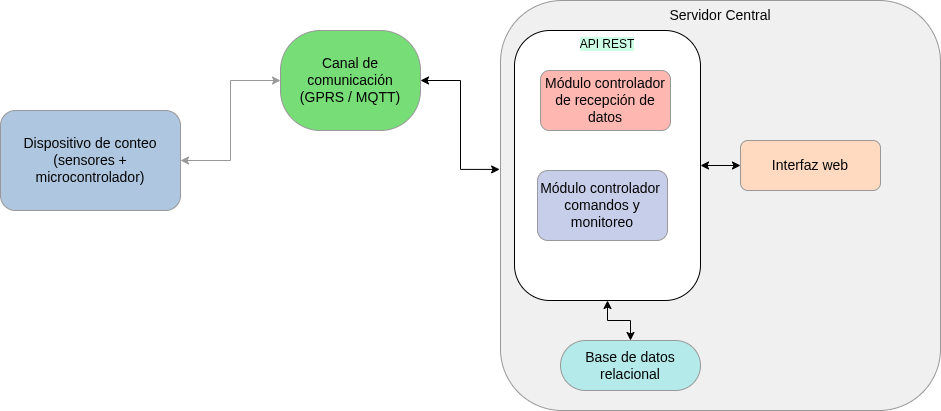
\includegraphics[width=\linewidth]{./Figures/diagBloques.png}
  \caption{Diagrama en bloques del sistema.}
  \label{fig:diag_bloques}
\end{figure}












